\documentclass[12pt]{article}
\usepackage[utf8]{inputenc}
\usepackage[T1]{fontenc}
\usepackage{graphicx}
\usepackage{xcolor}
\usepackage{hyperref}
\usepackage[english]{babel}

%%novalidate

\usepackage{tikz}
\usepackage{calc}
\usepackage{booktabs}
%\usepackage{hyperref}

% colors
\definecolor{color1}{HTML}{000060}
%\definecolor{color1}{HTML}{8C260F}
\definecolor{color2}{HTML}{333333}


% fonts
\usepackage{fontspec}
\defaultfontfeatures{Mapping=tex-text}
\setmainfont
[BoldFont=Lato-Bold.ttf,
ItalicFont=Lato-Italic.ttf,
BoldItalicFont=Lato-BoldItalic.ttf]
{Lato-Regular.ttf}
\newfontfamily\headingfont[ItalicFont=Lato-BlackItalic.ttf]{Lato-Black.ttf}
%%%

\usepackage{geometry}
\geometry{a4paper,
hmargin=20mm,vmargin=20mm,
head=0ex,foot=3ex}

\linespread{1.3}

\usepackage[hang]{caption}
\DeclareCaptionFormat{upper}{#1#2\uppercase{#3}\par}
\captionsetup{labelfont={bf,color=color2},textfont={normalsize,color=color2},format = upper,figurename=FIGURE,tablename=TABLE}

%%% fancy sections
\usepackage{titlesec}
%\titleformat{\chapter}{\headingfont\LARGE\bfseries\scshape\color{color1}}{\thechapter}{1em}{}[\titlerule]
\titleformat{\section}{\color{color1}\headingfont\Large\bfseries\uppercase}{\thesection}{1em}{}[\titlerule]
\titleformat{\subsection}{\color{color1}\headingfont\large\bfseries\uppercase}{\thesubsection}{1em}{}
\titleformat{\subsubsection}{\color{color1}\headingfont\bfseries\uppercase}{\thesubsubsection}{1em}{}
%%%

% head and foot
\usepackage{fancyhdr}
\pagestyle{fancy}
\lhead{}
\chead{}
\makeatletter
\rhead{\color{color2}\@date}
\makeatother
\newlength{\myheight}
\lfoot{
\settoheight{\myheight}{\thepage}
\raisebox{-2ex-0.5\myheight}{
\includegraphics[height=4ex]{logo}}
}
\cfoot{\color{color2}VIET NGUYEN - Aalto University}
\rfoot{\color{color2}\thepage}
\renewcommand\headrulewidth{0pt}
\renewcommand\footrulewidth{0pt}

%%% picture on cover page
\usepackage{eso-pic}
\newcommand\BackgroundPic{%
\put(0,0){%
\parbox[b][\paperheight]{\paperwidth}{%
\vfill
\centering

\includegraphics[width=\paperwidth,height=\paperheight,%
keepaspectratio]{cover}%
\vfill
}}}
%%%
% custom titlepage
\makeatletter
\renewcommand{\maketitle}{
\thispagestyle{empty}
\AddToShipoutPicture*{\BackgroundPic}
\ClearShipoutPicture
%
\phantom{a}
\vfill
\phantom{a}\hfill
\begin{tabular}[c]{@{}p{0.7\textwidth}@{}}
      \color{white}\headingfont\LARGE\@title\\[1em]
      \color{white}\headingfont\Large\@author\\[2em]
\end{tabular}
%
\clearpage
}
\makeatother
%%%


%%% fancy boxes
\usepackage{tcolorbox}
\usepackage{wrapfig}
\def\fullboxbegin{
\bigskip
\begin{tcolorbox}[colback=color1,colframe=color1,coltext=white,arc=0mm,boxrule=0pt]
}
\def\fullboxend{\end{tcolorbox}\medskip}
%
\def\leftboxbegin{
\begin{wrapfigure}{l}{0.5\textwidth}
\begin{tcolorbox}[colback=color1,colframe=color1,coltext=white,arc=0mm,boxrule=0pt]
}
\def\leftboxend{
\end{tcolorbox}
\end{wrapfigure}
}
%
\def\rightboxbegin{
\begin{wrapfigure}{r}{0.5\textwidth}
\begin{tcolorbox}[colback=color1,colframe=color1,coltext=white,arc=0mm,boxrule=0pt]
}
\def\rightboxend{
\end{tcolorbox}
\end{wrapfigure}
}
%
\newcounter{frames}
\def\frameboxbegin#1{
\bigskip
\refstepcounter{frames}
\begin{tcolorbox}[colback=white,colframe=color1,arc=0mm,title={\MakeUppercase{\textbf{Frame \arabic{frames}}: #1}}]
}
\def\frameboxend{
\end{tcolorbox}
}
%%%

\usepackage{lipsum}
\usepackage[nottoc]{tocbibind}

%%%%%%%%%%%%%%%
% Title Page
\title{Application of AI in telecom industry}
\author{Viet Nguyen \newline Aalto University}
\date{}
%%%%%%%%%%%%%%%

\begin{document}
\maketitle
% Need to add this
% https://www.techemergence.com/telecom-machine-learning-applications/% And make image
\tableofcontents
\clearpage

%: section 1: general strats, benefit. 2: ai research 3 : ai application alrdy done 
\section{Telecom industry is being disrupted by AI}
\noindent The trend of big telecom companies buying media companies for their content is continuing and even accelerating. %\cite{FastCompany}

\noindent Machine Learning and Deep Learning are a growing and diverse fields of Artificial Intelligence (AI) which studies algorithms that are capable of automatically learning from data and making predictions based on data. Machine Learning and Deep Learning are two of the most exciting technological areas of AI today. Each week there are new advancements, new technologies, new applications, and new opportunities. That's why Telecom companies should keep pace with all these exciting developments

\section{AI Research in Telecoms - network management}
\noindent In order to take advantage of exponential power of artificial intelligence, research is the first place to look. Here are some ideas I collected from many important research papers which relate telecommunications industry.
\subsection{Orchestration}
\noindent A fully NFV-enabled network will ultimately be controlled by a single NFV
orchestrator (NFVO). Accurately predicting network trends could lead to significant
improvements in network health and could significantly improve user experience.
\subsection{SDN controller}
\noindent Traffic through telco networks will ultimately be controlled by a centralized
SDN controller that may be augmented by AI functionality. This will allow the efficient and
proactive routing of traffic so that network outages are minimized and faults bypassed.
\subsection{Network deployment and optimization}
\noindent Self-optimizing networks (SONs) are a key pillar for 5G
and NFV networks. AI may be used to continuously optimize the configuration of a telco
network according to traffic volumes, user behavior, and other parameters. Network
deployments may also be further improved by AI, which will be used to predict traffic patterns
and forecast user trends.
\section{AI Research in Telecoms - CUSTOMER RELATION}
\noindent In order to take advantage of exponential power of artificial intelligence, research is the first place to look. Here are some ideas I collected from many important research papers which relate telecommunications industry.
\subsection{Detecting Fraudulent Calls}
\noindent Telecommunications has experienced dramatic expansion due to the rise of mobile phone adoption. However, with increasing number of mobile phone users comes increasing amount of phone fraud. Mobile communication fraud is common since it is easy to get a subscription using fake ID and mobile terminals are not bound to physical locations. These factors allow fraudsters to profit with relatively low risk of getting caught. Mobile phone fraud is defined as the unauthorised use, tampering or manipulation of a mobile phone or service.\cite{fraud1}
\subsection{Predicting Customer Churn}
\noindent Churn models aim to identify early churn signals and recognize customers with an increased likelihood to leave voluntarily. “Over the last decade there has been increasing interest (in fraud detection) studies in areas including telecommunication industry.” \cite{churn1}
\noindent We can also employ various AI techniques to classify customer’s segmentation based on Customer’s Age Group, VIP Status, Spend Status and Customer Length of Service \cite{segment1}

By predicting when customers will churn, telecommunications and media companies can save money. For example, the telecom industry suffered losses of around £953 million (\$1.56 billion USD) in 2011, a based on an average loss of 2.4 per cent against the total operator reported revenue of £39.7 billion (\$64.9 billion USD) \cite{fraud2}. In 2016, Telus lost 1.21\% of subscribers per month due to churn. \cite{telus}

\subsection{Predicting Customer Experience}
\noindent Real-time understanding of customer experience and satisfaction is one of the key competitive advantages of telecommunication companies. Telcos deal with large amounts of information generated by it’s users every day. For example: “mobile data traffic is forecasted to reach 24.3 Exabytes per month by 2019, which corresponds to a 10-fold growth from 2014 to 2019”. Such large and fast mobile data makes it harder for telcos to extract customer insights in a timely enough manner to react to potential causes of poor customer experience. \cite{churn2}

Many AI and machine learning techniques will enable us to classify customer experiences based on data feeds, customer care calls, spatial distribution, and temporal distribution effectively and accurately.


\subsection{intelligent agents}
\noindent Another application area in telecoms is the use of intelligent agents, also called digital assistants or
chatbots. Digital assistants have been in existence for some years but we are concerned here with the
new generation powered by AI. Sophisticated chatbots listen to speech, perform natural language
understanding, and respond with a simulated human-like voice (there are also purely text-based
chatbots), and are used to provide an automated service for answering consumer questions or firstline
customer support services. The speech recognition and natural language processing in these
machines has improved dramatically in the last few years.

\section{How leaders in telecom industry employ AI}
\noindent There are many companies that are already using AI, machine learning and deep learning in their products and services. Here are some of our industry favourites.

\subsection{Telus}
\begin{itemize}
	\item Telus uses machine learning to monitor “noise rise from more than 20,000 cell towers to increase service and device availability and mean time to repair (MTTR)” using Splunk . TELUS provides wireless services across Canada with a network of over 20,000 cell towers. Early identification and remediation of difficult-to-detect network incidents is crucial to maintaining customer satisfaction. TELUS uses Splunk machine learning to “reduce cell tower downtime and increase service availability.” \cite{splunk}
\end{itemize}

\subsection{CenturyLink}
\begin{itemize}
	\item CenturyLink offers Data \& Analytics Services as part of it’s IT Services \& Consulting \cite{centurylink}
\end{itemize}

\subsection{Comcast}
\begin{itemize}
	\item Comcast holds PHLAI — “a technical conference for engineers and professionals interested in and working with machine learning and artificial intelligence.” \cite{h2o1}
	\item Comcast used H2O's machine learning to improve X1 by XFINITY features, improve customer care, improve customer experience, create more resilient \& reliable products \cite{h2o1}, prevent avoidable truck rolls (an appointment at a customer’s home or business), predict trending content to offer personalized suggestions and browsing options for TV audiences, develop customer experience metric, improve product resiliency \cite{h2o2}
	\item Comcast Applied Artificial Intelligence Research team uses NLP, computer vision, and machine learning (with a focus on deep learning) to invent “the technological foundations for the Xfinity experiences of the future” 
	\item Comcast uses Apache Spark to “detect anomalies in customer activity that may indicate service interruptions” by analyzing “usage clickstreams and contract events such as telesales and emails”
\end{itemize}

\subsection{AT\&T}
\begin{itemize}
	\item AT\&T Big Data Research uses machine learning, data visualizations to “invent the new technologies and build platforms which empower AT\&T’s Big Data initiatives” \cite{att}
	\item AT\&T Intelligent Services and Platform Research uses artificial intelligence, human/machine interaction to “conduct research that empowers the next generation of autonomous and interactive services” \cite{att}
	\item AT\&T Labs uses artificial intelligence, networking and data analytics to develop “machine learning and massive data modeling platforms” \cite{att}
\end{itemize}

\subsection{Verizon}
\begin{itemize}
	\item Exponent by Verizon offers “software solutions built specifically to meet the needs of the global carrier community”. Exponent offers Artificial Intelligence Platform “designed to assist carriers to unlock and monetize their wealth of data through the application of advanced machine learning techniques, deep analytics, and artificial intelligence” \cite{verizon1}
	\item Verizon uses Apache Hadoop and Apache Spark for big data infrastructure \cite{verizon2}
\end{itemize}

\subsection{Nokia}
\noindent Nokia offers machine learning-powered customer experience solutions via Customer Care Solutions. Solutions include: reduction of time a customer is on a phone, improvement of solving cases on first contact, escalations reduction, call reduction due to successful self-help/IVR, reduction of propensity to call (PTC), repeat call reduction, improvement of NIPS/recommend to others, truck rolls reduction due to self-care, and improvement of call prediction \cite{nokia}.



%\section{a recommended strategy for AI}
%\noindent It is suggested that telecom organization should formulate a research for internal use that evaluates the potential of AI in various application areas, such as big data analysis, natural speech understanding, speech
%translation, and system optimization.
%
%\noindent it will be useful to look at forecasting the growth in AI improvement and how this will
%impact your domain. AI systems are likely to continue to evolve as new AI hardware accelerators enter
%the market and create new opportunities and improvements in AI algorithms. 
%
%\noindent The next step is to decide on what type of AI software capability to create in your organization:
%\begin{itemize}
%	\item Create in-house team and hire people
%	\item Make acquisition(s)
%	\item 
%\end{itemize}


%\subsection{Pictures used}
%
%\noindent
%Cover picture filename (in titlepage): \texttt{cover}\\
%Logo filename (in foot): \texttt{logo}
%
%\subsection{Boxes}

%\begin{verbatim}
%\fullboxbegin
%Content
%\fullboxend
%\end{verbatim}
%
%\begin{verbatim}
%\leftboxbegin
%Content
%\leftboxend
%\end{verbatim}
%
%\begin{verbatim}
%\rightboxbegin
%Content
%\rightboxend
%\end{verbatim}
%
%\begin{verbatim}
%\frameboxbegin{Frame Title}
%Content
%\frameboxend
%\end{verbatim}

%\newpage
%
%\section{First section}
%\lipsum[1]
%
%\fullboxbegin
%\lipsum[1]
%\fullboxend
%
%\lipsum[1]
%
%\subsection{First subsection}
%\lipsum[1]
%
%\leftboxbegin
%Lorem ipsum dolor sit amet, consectetuer adipiscing elit. Ut purus elit, vestibulum ut, placerat ac, adipiscing vitae, felis. Curabitur dictum gravida mauris. Nam arcu libero, nonummy eget, consectetuer id, vulputate a, magna. Donec vehicula augue eu neque. 
%\leftboxend
%
%\lipsum[1-2]
%
%\rightboxbegin
%\begin{itemize}
% \item Lorem ipsum
% \item Lorem ipsum
%\end{itemize}
%\rightboxend
%
%\lipsum[1]
%
%\subsubsection{First subsubsection}
%
%This document is an example of BibTeX using in bibliography management. Three items are cited: \textit{The \LaTeX\ Companion} book \cite{latexcompanion}, the Einstein journal paper \cite{einstein}, and the Donald Knuth's website \cite{knuthwebsite}. The \LaTeX\ related items are \cite{latexcompanion,knuthwebsite}.
%
%
%\begin{figure}[!h]
%\centering
%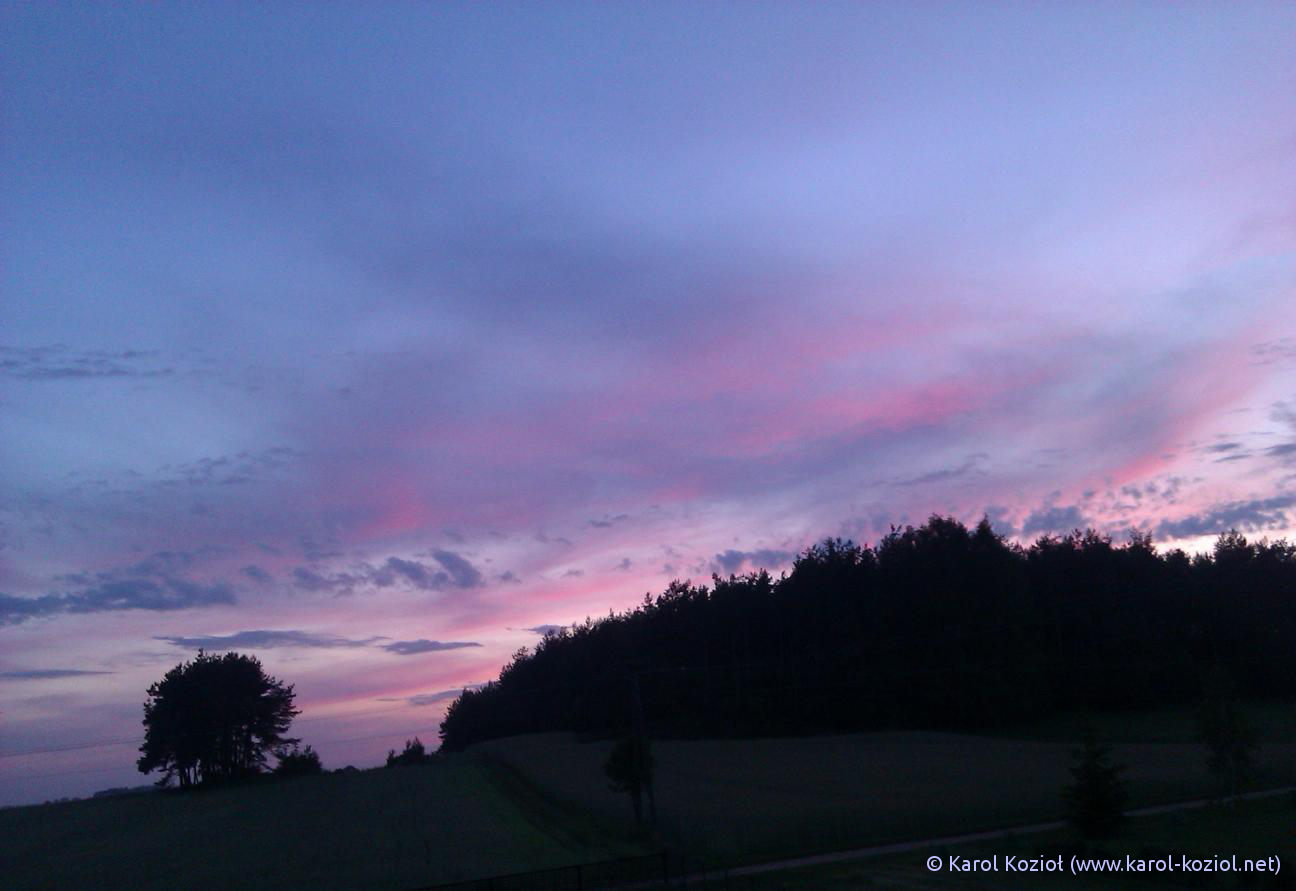
\includegraphics[width=0.5\textwidth]{sky.jpg}
%\caption{The sky is the limit.}
%\end{figure}
%
%\section*{Unnumbered section}
%\lipsum[1]
%
%\begin{figure}[!h]
%\centering
%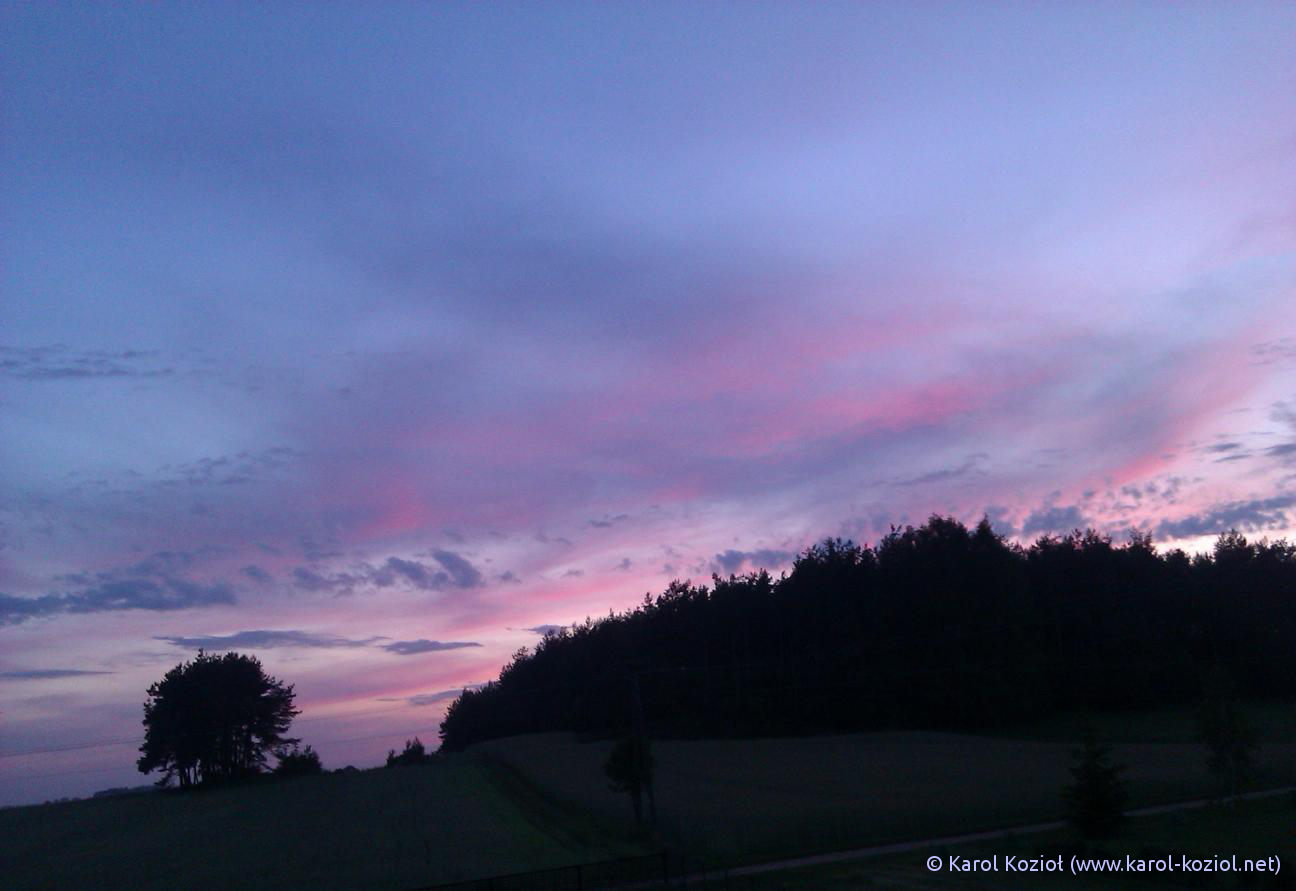
\includegraphics[width=0.5\textwidth]{sky.jpg}
%\caption*{The sky is the limit.}
%\end{figure}
%
%\section{Second section}
%
%\lipsum[1]
%\begin{table}[!h]
%\centering
%\caption{Sample table.}
%\begin{tabular}{cccc}
%\toprule
%Value 1 & Value 2 & Value 3 & Value 4\\
%\midrule
% odd     & odd   & odd & 1.00 \\
% even    & even  & even& 1.00 \\
% odd     & odd   & odd & 1.00 \\
% even    & even  & even& 1.00 \\
%\bottomrule
%\end{tabular}
%\end{table}
%
%\lipsum[1]
%
%\frameboxbegin{Sample frame}
%\lipsum[1]
%\frameboxend

%\bibliographystyle{unsrt}
%\bibliography{sample}

\section{}
\noindent

\begin{thebibliography}{9}
	\bibitem{fraud1}
	Subudhi, S., \& Panigrahi, S, 
	\href{https://dl.acm.org/citation.cfm?id=2898531}{Use of fuzzy clustering and support vector machine for detecting fraud in mobile telecommunication networks}, 
	International Journal of Security and Networks, 
	11(1–2), 3–11,
	2016
	
		\bibitem{fastcompany}
	MARK SULLIVAN
	\href{https://www.fastcompany.com/3068696/why-2017-will-be-a-huge-year-for-telecom-and-media-mergers}{Why 2017 Will Be A Huge Year For Telecom And Media Mergers}, 
	Fast Company,
	24 August 2017
	
	\bibitem{churn1}
	Vafeiadis, T., Diamantaras, K. I., Sarigiannidis, G., \& Chatzisavvas, K. C, 
	\href{http://www.sciencedirect.com/science/article/pii/S1569190X15000386}{A comparison of machine learning techniques for customer churn prediction}, 
	Simulation Modelling Practice and Theory, 
	55, 1–9,
	2015
	
	\bibitem{segment1}
	Dullaghan, C., \& Rozaki, E. 
	\href{https://arxiv.org/abs/1702.02215}{Integration of Machine Learning Techniques to Evaluate Dynamic Customer Segmentation Analysis for Mobile Customers}, 
	arXiv preprint arXiv:1702.02215, 
	2017
	
	\bibitem{fraud2}
	Gareth Pritchard,  
	\href{http://www.unionstreet.uk.com/telecoms-fraud-minimizing-the-risk/}{Telecoms fraud: minimising the risk}, 
	Union Street, 
	July 2017	
	
	\bibitem{ml1}
	Kepes, B.  
	\href{http://www.computerworld.com/article/3125517/big-data/splunk-ups-the-machine-learning-ante.html}{Splunk ups the machine-learning ante}, 
	Computerworld, 
	July 2017
	
	\bibitem{splunk}
	\href{https://www.splunk.com/en_us/products/splunk-enterprise/features/machine-learning.html}{Machine Learning}, 
	Splunk Enterprise , 
	July 2017
	
	
	
	\bibitem{h2o1}
	Ambati.  
	\href{https://www.slideshare.net/0xdata/h2o-world-machine-learning-at-comcast-andrew-leamon-chushi-ren}{H2O World — Machine Learning at Comcast}, 
	Comcast,
	2017
	
	\bibitem{h2o2}
	Kepes, B.  
	\href{http://www.h2o.ai/wp-content/uploads/2017/03/Case-Studies_Comcast.pdf}{Operationalizing Machine Learning at Comcast}, 
	Comcast, 
	2017
	
	\bibitem{att}
	\href{http://about.att.com/innovationblog/next_att_labs}{What’s Next at AT\&T Labs? AI Set to Revolutionize the Network}, 
	AT\&T, 
	2016
	
	\bibitem{verizon1}
	\href{http://www.exponentplatforms.com/verizon-launches-exponent}{Verizon Launches Exponent, a New Technology and Business Venture Designed to Accelerate Growth for Global Carriers.}, 
	Exponentplatforms.com, 
	2017
	
	\bibitem{verizon2}
	\href{http://mmds-data.org/presentations/2014/srivastava_mmds14.pdf}{Large-Scale Machine Learning at Verizon}, 
	MMDS, 
	2014
	
	\bibitem{nokia}
	\href{https://networks.nokia.com/solutions/customer-care}{Nokia - Customer Care Solutions}, 
	Nokia Networks, 
	2017
	
	\bibitem{telus}
	\href{http://about.telus.com/investors/annualreport2016/?lang=en}{TELUS Annual Report 2016}, 
	Telus, 
	2016
	
	\bibitem{churn2}
	Diaz-Aviles, E., Pinelli, F., Lynch, K., Nabi, Z., Gkoufas, Y., \& Bouillet, E. et al. 
	\href{https://arxiv.org/abs/1508.02884}{Towards Real-time Customer Experience Prediction for Telecommunication Operators}, 
	Arxiv.org, 
	2015
	
	\bibitem{netflix1}
	\href{https://medium.com/netflix-techblog/content-popularity-for-open-connect-b86d56f613b}{Content Popularity for Open Connect}, 
	Netflix TechBlog, 
	2017
	
	\bibitem{netflix2}
	Gomez-Uribe, Carlos A., and Neil Hunt.
	\href{https://medium.com/netflix-techblog/content-popularity-for-open-connect-b86d56f613b}{The netflix recommender system: Algorithms, business value, and innovation}, 
	ACM Transactions on Management Information Systems (TMIS), 
	2016

	\bibitem{centurylink}
	\href{http://www.centurylink.com/business/enterprise/it-consulting/data-analytics.html}{Data \& Analytics Services - CenturyLink}, 
	Centurylink.com, 
	2017


\end{thebibliography}
\end{document}          
